\documentclass[8pt,red]{beamer}
\usepackage{amsmath,amsthm,amsfonts,amssymb,amsbsy}
\usepackage{stmaryrd} 
\usepackage{subeqnarray}

\usepackage{cases}

\usepackage{pifont}

\usepackage{fancyhdr}

\usepackage{lastpage}


\usepackage{graphicx}
%\usepackage{subfloat}
\usepackage{rotating}
\usepackage{tikz}

\usetikzlibrary{arrows}
\usetikzlibrary{calc}
\usepackage{mathtools}

% \usepackage{algorithm}
% \usepackage{algorithmic}

\usepackage{siunitx}
\usepackage{subfig,float}


%% Symbole de fraction
\newcommand{\Frac}[2]{{\displaystyle \frac{\displaystyle #1}{\displaystyle #2}}}
\newcommand{\Prac}[2]{\displaystyle \genfrac{(}{)}{}{}{\displaystyle #1}{\displaystyle #2}}
\newcommand{\Crac}[2]{\displaystyle \genfrac{[}{]}{}{}{\displaystyle #1}{\displaystyle #2}}

\newcommand{\norme}[1]{\|#1\|}


\newcommand{\HRule}{\rule{\linewidth}{1mm}}

% Fonction math�matiques

\newcommand{\transposee}[1]{{\vphantom{#1}}^{\text{\tiny{\textsf T}}}{#1}}
%\newcommand{\argmin}{\mathop{\mathrm{argmin}}}
\newcommand{\argminn}{\mathop{\mathrm{argmin}}}
\newcommand{\lexicomin}{\mathop{\mathrm{lexicomin}}}
%\newcommand{\arg}{\mathop{\mathrm{arg}}}



\DeclareMathOperator{\rot}{rot}
\DeclareMathOperator{\sh}{sh}
\DeclareMathOperator{\ch}{ch}
%\DeclareMathOperator{\th}{th}
\DeclareMathOperator{\arcsh}{arcsh}
\DeclareMathOperator{\argth}{argth}
\DeclareMathOperator{\sign}{sign}




%%The Principal Value Integral symbol
\def\Xint#1{\mathchoice
   {\XXint\displaystyle\textstyle{#1}}%
   {\XXint\textstyle\scriptstyle{#1}}%
   {\XXint\scriptstyle\scriptscriptstyle{#1}}%
   {\XXint\scriptscriptstyle\scriptscriptstyle{#1}}%
   \!\int}
\def\XXint#1#2#3{{\setbox0=\hbox{$#1{#2#3}{\int}$}
     \vcenter{\hbox{$#2#3$}}\kern-.5\wd0}}
\def\ddashint{\Xint=}
\def\dashint{\Xint-}



% macro pour les symbols d'ensemble
%\nbOne
\def\nbOne{{\mathchoice{\rm 1\mskip-4mu l}{\rm 1\mskip-4mu l} {\rm 1 \mskip-4.5mu l}{\rm 1\mskip-5mu l}}}
%
%%  Les ensembles de nombres  C. Fiorio (fiorio�at�math.tu-berlin.de) 
%
\def\nbR{\ensuremath{\mathrm{I\!R}}} % IR
\def\nbN{\ensuremath{\mathrm{I\!N}}} % IN
\def\nbF{\ensuremath{\mathrm{I\!F}}} % IF
\def\nbH{\ensuremath{\mathrm{I\!H}}} % IH
\def\nbK{\ensuremath{\mathrm{I\!K}}} % IK
\def\nbL{\ensuremath{\mathrm{I\!L}}} % IL
\def\nbM{\ensuremath{\mathrm{I\!M}}} % IM
\def\nbP{\ensuremath{\mathrm{I\!P}}} % IP
%
% \nbOne : 1I : symbol one
\def\nbOne{{\mathchoice {\rm 1\mskip-4mu l} {\rm 1\mskip-4mu l}
{\rm 1\mskip-4.5mu l} {\rm 1\mskip-5mu l}}}
%
% \nbC   :  Nombres Complexes
\def\nbC{{\mathchoice {\setbox0=\hbox{$\displaystyle\rm C$}%
\hbox{\hbox to0pt{\kern0.4\wd0\vrule height0.9\ht0\hss}\box0}}
{\setbox0=\hbox{$\textstyle\rm C$}\hbox{\hbox
to0pt{\kern0.4\wd0\vrule height0.9\ht0\hss}\box0}}
{\setbox0=\hbox{$\scriptstyle\rm C$}\hbox{\hbox
to0pt{\kern0.4\wd0\vrule height0.9\ht0\hss}\box0}}
{\setbox0=\hbox{$\scriptscriptstyle\rm C$}\hbox{\hbox
to0pt{\kern0.4\wd0\vrule height0.9\ht0\hss}\box0}}}}
%
% \nbQ   : Nombres Rationnels Q
\def\nbQ{{\mathchoice {\setbox0=\hbox{$\displaystyle\rm
Q$}\hbox{\raise
0.15\ht0\hbox to0pt{\kern0.4\wd0\vrule height0.8\ht0\hss}\box0}}
{\setbox0=\hbox{$\textstyle\rm Q$}\hbox{\raise
0.15\ht0\hbox to0pt{\kern0.4\wd0\vrule height0.8\ht0\hss}\box0}}
{\setbox0=\hbox{$\scriptstyle\rm Q$}\hbox{\raise
0.15\ht0\hbox to0pt{\kern0.4\wd0\vrule height0.7\ht0\hss}\box0}}
{\setbox0=\hbox{$\scriptscriptstyle\rm Q$}\hbox{\raise
0.15\ht0\hbox to0pt{\kern0.4\wd0\vrule height0.7\ht0\hss}\box0}}}}
%
% \nbT   : T
\def\nbT{{\mathchoice {\setbox0=\hbox{$\displaystyle\rm
T$}\hbox{\hbox to0pt{\kern0.3\wd0\vrule height0.9\ht0\hss}\box0}}
{\setbox0=\hbox{$\textstyle\rm T$}\hbox{\hbox
to0pt{\kern0.3\wd0\vrule height0.9\ht0\hss}\box0}}
{\setbox0=\hbox{$\scriptstyle\rm T$}\hbox{\hbox
to0pt{\kern0.3\wd0\vrule height0.9\ht0\hss}\box0}}
{\setbox0=\hbox{$\scriptscriptstyle\rm T$}\hbox{\hbox
to0pt{\kern0.3\wd0\vrule height0.9\ht0\hss}\box0}}}}
%
% \nbS   : S
\def\nbS{{\mathchoice
{\setbox0=\hbox{$\displaystyle     \rm S$}\hbox{\raise0.5\ht0%
\hbox to0pt{\kern0.35\wd0\vrule height0.45\ht0\hss}\hbox
to0pt{\kern0.55\wd0\vrule height0.5\ht0\hss}\box0}}
{\setbox0=\hbox{$\textstyle        \rm S$}\hbox{\raise0.5\ht0%
\hbox to0pt{\kern0.35\wd0\vrule height0.45\ht0\hss}\hbox
to0pt{\kern0.55\wd0\vrule height0.5\ht0\hss}\box0}}
{\setbox0=\hbox{$\scriptstyle      \rm S$}\hbox{\raise0.5\ht0%
\hboxto0pt{\kern0.35\wd0\vrule height0.45\ht0\hss}\raise0.05\ht0%
\hbox to0pt{\kern0.5\wd0\vrule height0.45\ht0\hss}\box0}}
{\setbox0=\hbox{$\scriptscriptstyle\rm S$}\hbox{\raise0.5\ht0%
\hboxto0pt{\kern0.4\wd0\vrule height0.45\ht0\hss}\raise0.05\ht0%
\hbox to0pt{\kern0.55\wd0\vrule height0.45\ht0\hss}\box0}}}}
%
% \nbZ   : Entiers Relatifs Z
\def\nbZ{{\mathchoice {\hbox{$\sf\textstyle Z\kern-0.4em Z$}}
{\hbox{$\sf\textstyle Z\kern-0.4em Z$}}
{\hbox{$\sf\scriptstyle Z\kern-0.3em Z$}}
{\hbox{$\sf\scriptscriptstyle Z\kern-0.2em Z$}}}}
%%%% fin macro %%%%



\newcommand{\putidx}[1]{\index{#1}\textit{#1}}
% macro pour r�f�rencer les �quations


\newcommand{\reffig}[1]{({\it cf} figure : \ref{#1})}
\newcommand{\refann}[1]{({\it cf} Annexe : \ref{#1})}


%\definecolor{darkgray}{gray}{.25}
\definecolor{gray}{gray}{.5}
\definecolor{lightgray}{gray}{.75}
%\definecolor{gradbegin}{rgb}{0,1,1}
%\definecolor{gradend}{rgb}{0,.1,.95}
%\newcommand{\newtexte}[1]{\textcolor{darkgray} {#1}}
\newcommand{\newtexte}[1]{{#1}}% macro pour les varibales favorites
% normal tangent
\def\n{{\hbox{\tiny{N}}}}
\def\t{{\hbox{\tiny{T}}}}
\def\ss{{\hbox{\tiny{S}}}}
\def\nt{\hbox{\tiny{NT}}}
\def\nsf{\hbox{\tiny{\textsf N}}}
\def\tsf{\hbox{\tiny{\textsf T}}}
\def\sigman{\sigma_{\n}}
\def\sigmat{\sigma_{\t}}
\def\sigmant{\sigma_{\nt}}
\def\epsn{\epsilon_{\n}}
\def\epst{\epsilon_{\t}}
\def\epsnt{\epsilon_{\nt}}
\def\eps{\epsilon}
\def\veps{\varepsilon}
\def\sig{\sigma}
\def\Rn{R_{\n}}
\def\Rt{R_{\t}}
\def\cn{c_{\n}}
\def\Cn{C_{\n}}
\def\ct{c_{\t}}
\def\Ct{C_{\t}}
\def\un{u_{\n}}
\def\ut{\buu_{\t}}
\def\uut{u_{\t}}
\def\unc{u_{\n}^c}
\def\utc{\buu_{\t}^c}
\def\vn{v_{\n}}
\def\vt{v_{\t}}
\def\rr{\hbox{\tiny{\textsf R}}}
\def\irr{\hbox{\tiny{\textsf{IR}}}}
\def\rn{r_{\n}}
\def\rt{\brr_{\t}}
\def\rnc{r_{\n}^c}
\def\rtc{\brr_{\t}^c}
\def\trn{\Tilde{r}_{\n}}
\def\trt{\Tilde{\brr}_{\t}}
\def\tr{\Tilde{\brr}}
\def\tv{\Tilde{\bvv}}
\def\vn{v_{\n}}
\def\vt{\bvv_{\t}}
\def\adh{\mathsf{adh}}
\def\adj{\hbox{\tiny{\textsf{adj}}}}
\def\adjc{\hbox{\tiny{\textsf{adjC}}}}
\def\adja{\hbox{\tiny{\textsf{adjA}}}}
\def\cc{\hbox{\tiny{\textsf C}}}
\def\ca{\hbox{\tiny{\textsf A}}}

%%    Unit�e
\def\mm{\,\mathsf{mm}}
\def\cm{\,\mathsf{cm}}
\def\m{\,\mathsf{m}}
\def\ms{\,\mathsf{m.s^{-1}}}
\def\mms{\,\mathsf{mm.s^{-1}}}
\def\Mpa{\,\mathsf{MPa}}
\def\Gpa{\,\mathsf{GPa}}
\def\Kg{\,\mathsf{Kg}}
\def\Hz{\,\mathsf{Hz}}
\def\kHz{\,\mathsf{kHz}}
\def\N{\,\mathsf{N}}
\def\kN{\,\mathsf{kN}}
\def\Nmmm{\,\mathsf{N.m^{-3}}}
\def\ds{d_{\hbox{\tiny{S}}}}
% domaines et frontieres
\def\om{\Omega}
\def\oma{\Omega^{\alpha}}
\def\omu{\Omega^1\cup \Omega^2}
\def\gc{\Gamma_c}
\def\omt{\omu \cup \gc}
% derivee partielle et gradient et divergence
\def\p{\partial}
\def\grad{\nabla}
\def\div{\mathop{\rm div}\nolimits}
%

%\DeclareTextSymbol{\deg}{T1}{6}
%\def\degre{\mathdegree}
%\newcommand{\degre}{\mathdegree}

\def\etc{\textit{etc}\ldots}
\newcommand{\mdegre}{\hbox{\text{\degre}}}

%\def\nscd{\textsf{\bfseries NSCD}}
%\def\nscd{\textsf{NSCD}}
\newcommand{\nscd}{\textsf{NSCD}}
%\Pisymbol{psy}{212} ou encore \Pisymbol{psy}{228}




%----------------------------------------------------------------------
%             Des chiffres avec des ronds autour
%----------------------------------------------------------------------
\def\nombrecercle#1{\def\taille{0.3}
                \put(0,0){#1}
                \put(0.08,0.08){\circle{\taille}}}



\def\ae#1{\stackrel{\mbox{\scriptsize a.e.}}{#1}}
%\def\argmin{\mathop{\rm argmin}}


\def\eqref#1{{\rm (\ref{#1})\/}}
\def\indicfon{\mathord{\rm i}}       %indicator function
\def\p{\mathord{\rm proj}}
\def\N{\mathord{\rm N}}
% \def\prosca#1#2{#1\cdot#2}
\def\prosca#1#2{\langle #1,#2\rangle}
\def\qedtext{\mbox{}\hfill$\Box$}
\def\qedmath{\eqno\Box}

\def\s{{$\mathcal{S}$}}
\def\somme{\mathop{\textstyle\sum}}
\def\somme{\mathop{\textstyle\sum}}
\def\submoins{_{\scriptscriptstyle-}}
\def\subplus{_{\scriptscriptstyle+}}
\def\T{\mathord{\rm T}}

%----------------------------------------------------------------------
%             Macro M Jean 
%----------------------------------------------------------------------

\def\Real{\mbox{I\hspace{-.15em}R}}
\def\Integer{\mbox{I\hspace{-.15em}N}}
\def\Bunit{\mbox{I\hspace{-.15em}B}}
\def\real{\mbox{\scriptsize I\hspace{-.15em}R}}
\def\bunit{\mbox{\scriptsize I\hspace{-.15em}B}}
\def\IL{\mbox{\scriptsize I\hspace{-.15em}L}}
\def\Indic{\mbox{\large $\psi$}}
\def\bfxi{\mbox{$\xi$ \hspace{-1.1em} $\xi$}}
%\def\bfXi{\mbox{$\Xi$ \hspace{-1.1em} $\Xi$}}
\def\RunR{\mathcal R}
\def\RunRN{\mathcal R_{N}}
\def\RunRT{\mathcal R_{T}}
\def\RunS{\mathcal S}
\def\RunSN{\mathcal S_{N}}
\def\RunST{\mathcal S_{T}}
\def\RunU{\mathcal U}
\def\RunUN{\mathcal U_{N}}
\def\RunUT{\mathcal U_{T}}
\def\RunUP{\mathcal U'}
\def\RunUPN{\mathcal U'_{N}}
\def\RunUPT{\mathcal U'_{T}}
\def\RunJ{\mathcal J}
\def\RunW{\mathcal W}
\def\RunF{f}
\def\RunFa{f_{1}}
\def\RunFb{f_{2}}
\def\RunFP{f'}
\def\RunV{v}
\def\RunVP{v'}
\def\EspF{\mathcal F}
\def\EspV{\mathcal V}
%%%%
\catcode`\�=13
\def�{\'e}
\catcode`\�=13
\def�{\`e}
\catcode`\�=13
\def�{\`a}
\catcode`\�=13
\def�{\c c}
\def\N{\mbox{I\hspace{ -.15em}N}}
\def\Z{\mbox{Z\hspace{ -.3em}Z}}
\def\Q{\mbox{l\hspace{ -.47em}Q}}
\def\R{\mbox{l\hspace{ -.15em}R}}
\def\F{\mbox{l\hspace{ -.15em}F}}
\def\E{\mbox{l\hspace{ -.15em}E}}
\def\LMGC90{{\small \it LMGC90 }}
\def\NSCD{{\small \it NSCD }}
\def\CHIC{{\small \it CHIC }}
\def\half{{\frac{_{1}}{^{2}}}}
\def\12T{{\frac{_{1}}{^{2T}}}}

\def\geq{\geqslant}
\def\leq{\leqslant}
\def\ge{\geqslant}
\def\le{\leqslant}


\begingroup
\count0=\time \divide\count0by60 % Hour
\count2=\count0 \multiply\count2by-60 \advance\count2by\time
% Min
\def\2#1{\ifnum#1<10 0\fi\the#1}
\xdef\isodayandtime{\the\year-\2\month-\2\day\space\2{\count0}:%
\2{\count2}}
\endgroup

%---------------------------------------------------------------------
%             Redaction note environnement B. Brogliato
%----------------------------------------------------------------------
\makeatletter

{\newtheorem{ndr1bb}{\textbf{\textsc{Redaction note B.B.}}}[section]}

\newenvironment{ndrbb}%
{%
\noindent\begin{ndr1bb}\hrule\vspace{1em}%
\ttfamily\small
}%
{%
\begin{flushright}%
%\vspace{-1.5em}\ding{111}
\end{flushright}%
\vspace{-1.5em}\hrule
\end{ndr1bb}%
}
%----------------------------------------------------------------------
%             Redaction note environnement V.ACARY
%----------------------------------------------------------------------
% Faut etre fou pour s'amuser a pondre des notes pareilles

{\newtheorem{ndr1va}{\textbf{\textsc{\footnotesize Redaction note V.A.}}}[section]}

\newenvironment{ndrva}%
{%
\noindent\begin{ndr1va}\hrule\vspace{1em}%
\ttfamily\small \  \\
\noindent}%
{%
$ $ \\
\hrule
\end{ndr1va}%
}
\makeatother








% ----------------DEFINITIONS-----------------
% 

 \def\II{\mathop{{\rm I}\mskip-3.0mu{\rm I}}\nolimits}




% -----------------------------------
 \def\c{\mathop{{\rm 1}\mskip-10.0mu{\rm C}}\nolimits}
 \def\C{\mathop{{\rm 1}\mskip-10.0mu{\rm C}}\nolimits}
 \def\ZZ{\mathaccent23Z}
% 

\newcommand{\ie}{{\textit{i.e.}}}


%\def\sgn{\mbox{\rm sgn}}
\DeclareMathOperator{\sgn}{sgn}
\DeclareMathOperator{\proj}{proj}
\DeclareMathOperator{\prox}{prox}
\DeclareMathOperator{\argmin}{argmin}

\newcommand{\RR}{\mbox{\rm $I\!\!R$}}
\newcommand{\NN}{\mbox{\rm $I\!\!N$}}


% ---------------- MMC -----------------
% 

\newcommand{\contract}{{\,:\,}}

\newcommand{\scontract}{{\,{\Bar\otimes}\,}}
\newcommand{\tcontract}{{\,{\Bar{\Bar{\Bar\otimes}}}\,}}


\newcommand{\DP}[2]{\displaystyle \frac{\partial {#1}}{\partial {#2}}}

% %\newtheorem{definition}{Definition}
% \newtheorem{proposition}{Proposition}
% \newtheorem{lemma}{Lemma}

% \newtheorem{claim}{Claim}
% \newtheorem{remark}{Remark}
% \newtheorem{assumption}{Assumption}
% \newtheorem{example}{Example}
% \newtheorem{conjecture}{Conjecture}
% \newtheorem{corollary}{Corollary}
% \newtheorem{OP}{OP}
% \newtheorem{problem}{Problem}
% \newtheorem{theorem}{Theorem}


\def\dt{{\rm d}t}
\def\dv{{\rm d}v}
\def\di{{\rm d}i}
\def\dI{{\rm d}I}
\def\dU{{\rm d}U}


\def\nat{{\hbox{\tiny{nat}}}}
\def\nor{{\hbox{\tiny{nor}}}}
\def\fb{\hbox{\tiny{\textsf FB}}}
\def\vione{{\hbox{\tiny{vi-1}}}}
\def\vitwo{{\hbox{\tiny{vi-2}}}}
\def\qvitwo{{\hbox{\tiny{qvi-2}}}}
\def\acone{{\hbox{\tiny{ac-1}}}}
\def\actwo{{\hbox{\tiny{ac-2}}}}

%%% Local Variables:
%%% mode: latex
%%% TeX-master: "s"
%%% End:


\usepackage{wasysym}



\setbeamertemplate{theorem}[ams style]
\setbeamertemplate{theorems}[numbered]


%\input{../macro-mjean.tex}
% %hideothersubsections
% \usetheme[hideothersubsections,width=2.5cm]{Goettingen}
% %\useoutertheme[headline=empty]{miniframes}

\usetheme[]{Montpellier}
\makeatletter
\useoutertheme[height=0pt, width=0cm]{sidebar}
{\usebeamercolor{structure}}
\setbeamertemplate{sidebar canvas \beamer@sidebarside}[vertical shading][top=structure.fg!25,bottom=structure.fg!10]

%%% Local Variables: 
%%% mode: latex
%%% TeX-master: t
%%% End: 


\title{Nonsmooth Newton methods for frictional contact problems in flexible multi-body systems}
\author{V. Acary, M. Br\'emond, F. Dubois \\ INRIA Rh\^one--Alpes, Grenoble. \\ LMGC Montpellier}
\date{13\textsuperscript{eme} Colloque National en Calcul des structures \\ [2mm] \today}

\setbeamertemplate 
{footline} 
{\quad\hfill\strut\insertsection\quad--\quad\insertframenumber/\inserttotalframenumber\strut\quad\quad} 

\graphicspath{{../figure/}}

\includeonly{%
%  introduction,
  fc3d,
  %existence,
  numerics,
  comparison
}



%\newtheorem{defn}{Definition}
%\renewcommand{\thedefn}{\arabic{defn}}
% \newtheorem{thm}[defn]{Theorem}
% \newtheorem{corr}[defn]{Corollary}
% \newtheorem{ass}[defn]{Assumption}
% \newtheorem{lem}[defn]{Lemma}
% \newtheorem{rem}[defn]{Remark}
% \newtheorem{hypo}[defn]{Hypotheses}
% \newtheorem{exmp}[defn]{Example}
% \newtheorem{prop}[defn]{Proposition}
\newcommand{\diag}{\mbox{\rm diag}}
\newcommand{\co}{\overline{\mathit{co}}}
\newcommand{\rect}{\overline{\mathit{rect}}}
\newcommand{\newb}{g}

\renewcommand{\tr}[1]{\textcolor{red}{#1}}
\def\nat{{\hbox{\sf \tiny{nat}}}}
\def\ac{{\hbox{\tiny{ac}}}}
\def\mjtwo{{\hbox{\tiny{mj}}}}
\begin{document}

\frame{\titlepage
  \begin{center}
    
\includegraphics[height=0.1\textheight]{../figure/logo-inria.png}\\
    
\includegraphics[height=0.1\textheight]{../figure/logo-lmgc.jpg}
  \end{center}
  $$ $$
}


%\frame{\tableofcontents}

\begin{frame}
  \frametitle{Objectives}
  \begin{itemize}
  \item Computation methods for discrete frictional contact problems.
  \item Rigid multi-body systems:
    \begin{itemize}
    \item high order of hyperstaticity
    \item under-determinancy in the contact forces
    \item Projection/splitting methods (Jacobi, Gauss--Seidel) are robust but very slow
    \item Nonsmooth Newton methods fail
    \end{itemize}
  \item Flexible multi-body systems:
    \begin{itemize}
    \item low order of hyperstaticity
    \item Nonsmooth methods work efficiently.
    \end{itemize}
  \end{itemize}
  General interest in introducing flexibility in the model for computational efficiency.
\end{frame}


\section{The 3D frictional contact problem}
\label{Sec:fc3d}

\subsection{Signorini condition and Coulomb's friction}

\frame{
  \frametitle{Signorini's condition and Coulomb's friction} 
  \begin{minipage}[c]{0.49\linewidth}
    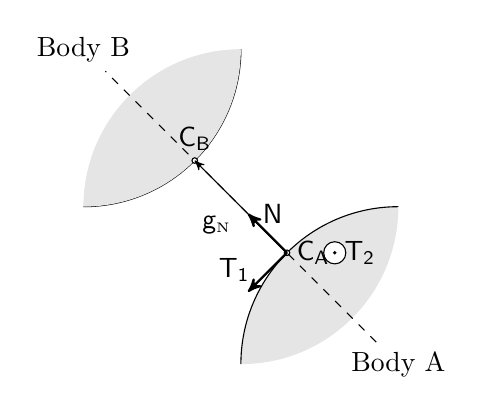
\begin{tikzpicture}[ scale=2,
      axis/.style={ ->, >=stealth'},
      normal/.style={ thick, ->, >=stealth'},
      important line/.style={very thick}, 
      dashed line/.style={dashed, thin},
      every node/.style={color=black},
      soldot/.style={only marks,mark=*},
      holdot/.style={fill=white,only marks,mark=*}
      ]
      % body
      \node (BodyA) at (1,-1) {Body A};
      \fill[gray!20] (1,0) arc (0:-90:1);
      \fill[gray!20] (1,0) arc (90:180:1);
      \draw (1,0) arc (90:180:1);

      \node (BodyB) at (-1,1) {Body B};
      \draw (0,1) arc (0:-90:1);
      \fill[gray!20] (0,1) arc (90:180:1);
      \fill[gray!20] (0,1) arc (0:-90:1);

      % local frame
      \def\nlength{0.35};
      \coordinate (CA)  at  ({1.0-sqrt(2)/2.0},{-1.0+sqrt(2)/2.0});
      \node[] at  (CA) [right] {$\sf C_A$};
      \draw[holdot]  (CA) circle(0.05em);
      \draw[normal] (CA) -- ($(CA)+({-\nlength*sqrt(2)/2.0},{+\nlength*sqrt(2)/2.0 })$) node [right] {$\,\sf N$};
      \draw[normal] (CA) -- ($(CA)+({-\nlength*sqrt(2)/2.0},{-\nlength*sqrt(2)/2.0 })$) node [above] {$\sf T_1\quad$};
      \draw[dashed line] (BodyA) -- (BodyB);
      \draw[holdot] ($(CA)+({\nlength*sqrt(3)/2.0},{0.0})$) circle(0.2em);
      \node at ($(CA)+({\nlength*sqrt(3)/2.0},{0.0})$) [right]{$\sf T_2$};
      \draw[soldot] ($(CA)+({\nlength*sqrt(3)/2.0},{0.0})$) circle(0.02em);
      
      \coordinate (CB)  at  ({-1.0+sqrt(2)/2.0},{1.0-sqrt(2)/2.0});
      \node at  (CB) [above] {$\sf C_B$};
      \draw[holdot]  (CB) circle(0.05em);

      \draw[axis] (CA) -- (CB) node[midway, below left ] {$\sf g_\n$} ;

      % \draw[axis] (0,-0.4) -- (0,0.4) node(yline)[right] {$\sgn(x)$};
      % % lines
      % \draw[important line] (-0.4,-0.3) -- (0.   ,-.3);
      % \draw[important line] (0.0,0.3) --(.4,.3)  ;
      % \coordinate (O) at (0.0, 0.05);
      % \draw[fill] (O) circle (0.03em);
      % \draw (0.0,0.05) node[right]{$a$};
      % \draw (0.0,0.3) node[left]{$1$};
      % \draw (0.0,-0.3) node[right]{$-1$};
      % \draw[holdot] (0.0,0.3) circle (0.03em);
      % \draw[holdot] (0.0,-.3) circle (0.03em);
    \end{tikzpicture}
  \end{minipage}
\begin{minipage}[c]{0.49\linewidth}
    \begin{itemize}
    \item gap function $ g_{\n} = (C_B-C_A) \sf N.$
    \item reaction forces $$ r =  r_\n {\sf N} + r_\t, \quad \text{ with  } r_\n \in \RR \text{ and } r_\t \in \RR^2.$$
    \item Signorini condition at position level
      $$  0 \leq g_{\n} \perp r_\n \geq 0. $$
    \item relative velocity
      $$u =  u_\n {\sf N} + u_\t, \quad \text{ with } u_\n \in \RR \text{ and } u_\t \in \RR^2.$$
    \item Signorini condition at velocity level
        $$\left\{\begin{array}{ll}
            0 \leq u_{\n} \perp r_\n \geq 0  &\text{ if } g_{\n} \leq 0 \\
            r_{\n} =0 &\text{ otherwise}.
          \end{array}\right.$$
    \end{itemize}

  \end{minipage}
}
\frame{
  \frametitle{Signorini's condition and Coulomb's friction} 
  \begin{block}{Modeling assumption}
   Let $\mu$ be the coefficient of friction.  Let us define the Coulomb friction cone $K$ which is chosen as the
    isotropic second order cone
    \begin{equation}
      \label{eq:CoulombCone}
      K = \{r \in \RR^3 \mid \|r_\t\| \leq \mu r_n\}.
    \end{equation}
    The Coulomb friction states
    \begin{itemize}
    \item for the \tr{sticking case} that
      \begin{equation}
        \label{eq:Coulom-stick}
        u_{\t} =0,\quad r \in K
      \end{equation}
    \item and for the \tr{sliding case} that
      \begin{equation}
        \label{eq:Coulom-slide}
        u_{\t}  \neq 0,\quad r \in \partial K, \exists\, \alpha > 0, r_\t = -\alpha u_\t.
      \end{equation}
    \end{itemize}
  \end{block}

  \begin{block}
    {Disjunctive formulation of the frictional contact behavior}
    \begin{equation}
      \label{eq:contact-disjunctive}
      \left\{\begin{array}{llr}
          r = 0  &\text{ if } g_{\n} > 0  & \text{(no contact)}\\
          r = 0,  u_\n \geq 0   &\text{ if } g_{\n} \leq 0 & \text{(take--off)} \\
          r \in K, u =0 &\text{ if } g_{\n} \leq 0 & \text{(sticking)}  \\
          r \in \partial K,u _\n=0,  \exists\,\alpha > 0, u_\t = -\alpha r_\t &\text{ if } g_{\n} \leq 0 & \text{(sliding)}  \\
        \end{array}\right.
    \end{equation}
  \end{block}
  

}

\frame{
  \frametitle{Signorini's condition and Coulomb's friction} 
  
  \begin{block}{Second Order Cone Complementarity (SOCCP) formulation \cite{DeSaxce92}}
  
    \begin{itemize}
    \item Modified relative velocity $\hat u \in \RR^3$ defined by
      \begin{equation}
        \label{eq:modified-velocity}
        \hat u = u +\mu \|u_\t\| \sf N.
      \end{equation}
    
    \item  Second-Order Cone Complementarity Problem (SOCCP) 
      \begin{equation}
        \label{eq:contact-SOCCP}
        K^\star \ni \hat u \perp r \in K
      \end{equation}
      if $ g_\n \leq 0 $ and $r=0$ otherwise.  The set $ K^\star $ is
      the dual convex cone to $K$ defined by
      \begin{equation}
        \label{eq:dual-cone}
        K^\star = \{u \in \RR^3 \mid  r^\top u \geq 0, \quad \text{for all } r \in K   \}.
      \end{equation}

    \end{itemize}
 \end{block}
    \vfill \small
    %\cite{DeSaxce92,Acary.Brogliato2008,ZAMM:ZAMM201000073}.

}
\frame{
  \frametitle{Signorini's condition and Coulomb's friction} 
   \begin{figure}[htbp]
  \centering
  \resizebox{!}{0.8\textheight}{\input{../figure/cone1-b.pdf_t}}
  \caption{Coulomb's friction and the modified velocity $\hat u$. The sliding case.}
  \label{fig:CoulombFrictionSlidingDeSaxce}
\end{figure} 
}

\subsection{3D frictional contact problems}


\frame{
  \frametitle{3D frictional contact problem} 
  \begin{block}{Multiple contact notation}
    For each contact $\alpha \in \{1,\ldots n_c\}$, we have
    \begin{itemize}
    \item the local velocity : $u^\alpha \in \RR^3$, and
      $$  u = [[u^\alpha]^\top, \alpha = 1\ldots n_c]^\top$$
    \item the local  reaction vector $r^\alpha\in \RR^3$    
      $$  r = [[r^\alpha]^\top, \alpha = 1\ldots n_c]^\top$$
    \item the local  Coulomb cone    $$K^{\alpha}  = \{r^\alpha, \|r^\alpha_\t \| \leq \mu^\alpha |r^\alpha_\n| \} \subset \RR^3$$
       and the set $K$ is the cartesian product of Coulomb's friction cone at each contact, that 
      \begin{equation}
        \label{eq:CC}
        K = \prod_{\alpha=1\ldots n_c} K^{\alpha} 
      \end{equation}
      and $K^\star$ is dual.
    \end{itemize} \end{block} 
}





\frame{
  \frametitle{3D frictional contact problems} 
  \begin{problem}[General discrete frictional contact problem]\label{prob:I}
  Given
  \begin{itemize}
    \item a symmetric positive definite matrix ${M} \in \nbR^{n \times n}$,
    \item a vector $ {f} \in \nbR^n$,
    \item a matrix  ${H} \in \nbR^{n \times m}$,
    \item a vector $w \in \RR^{m}$,
    \item a vector of coefficients of friction $\mu \in \RR^{n_c}$,
  \end{itemize}
find three vectors $ {v} \in \nbR^n$, $u\in\RR^m$ and $r\in \RR^m$, denoted by $\mathrm{FC/I}(M,H,f,w,\mu)$  such that
\begin{equation}\label{eq:soccp1}
  \begin{cases}
    M v = {H} {r} + {f} \\[2mm]
    u = H^\top v + w \\[2mm]
    \hat u = u + g(u) \\[2mm]
    K^\star \ni {\hat u} \perp r \in K
  \end{cases}
\end{equation}
with $g(u) = [[\mu^\alpha  \|u^\alpha_\t\| {\sf N}^\alpha]^\top, \alpha = 1\ldots n_c]^\top$. 
\qed
\end{problem}

}
\frame{
  \frametitle{3D frictional contact problems} 
  \begin{problem}[Reduced discrete frictional contact problem]\label{prob:II}
    Given
    \begin{itemize}
    \item a symmetric positive semi--definite  matrix ${W} \in \nbR^{m \times m}$,
    \item a vector $ {q} \in \nbR^m$,
    \item a vector $\mu \in \RR^{n_c}$ of coefficients of friction, 
    \end{itemize}
    find two vectors $u\in\RR^m$ and $r\in \RR^m$, denoted by $\mathrm{FC/II}(W,q,\mu)$  such that
    \begin{equation}\label{eq:soccp2}
      \begin{cases}
        u =Wr +q \\[2mm]
        \hat u =u + g(u) \\[2mm]
        K^\star \ni {\hat u} \perp r \in K
      \end{cases}
    \end{equation}
    with $g(u) = [[\mu^\alpha \|u^\alpha_\t\| {\sf N}^\alpha]^\top,  \alpha = 1\ldots n_c]^\top$.
    \qed
  \end{problem}
  
  \begin{block}{Relation with the general problem}
     $ W = H^\top M^{-1} H$ and $q = H^\top  M^{-1} f + w $.
  \end{block}
  
}
% \frame{
%   \frametitle{3D frictional contact problems} 
%   \begin{block}{Wide range of applications}

%     Origin of the linear relations~\nocite{Acary.Cadoux2013}.
%   $$  M v = {H} {r} + {f},\quad u = H^\top v + w$$
%   \begin{itemize}
%   \item Time--discretization of the discrete dynamical mechanical
%     system
%     \begin{itemize}
%     \item Event--capturing time--stepping schemes
%     \item Event--detecting time--stepping schemes (event-driven)
%     \end{itemize}
%   \item Time--discretization and space discretization of the elasto
%     dynamic problem of solids
%   \item Space discretization of the quasi--static problem of solids.
%   \end{itemize}
%   with a possible linearization (Newton procedure.)
% \end{block}
%    \ding{220}  These problems are really representative of a lot of applications.


% }

% \subsection{From the mathematical programming point of view}

% \frame{
%   \frametitle{From the mathematical programming point of view} 
%   \begin{block}{Nonmonotone and nonsmooth problem}
%     \begin{equation}
%       \label{eq:soccp3}
%       K^\star \ni Wr +q + g(Wr +q) \perp r \in K
%     \end{equation}
%     \begin{itemize}
%     \item if we neglect $g(\cdot)$, (\ref{eq:soccp3}) is a gentle
%       monotone SOCLCP that  is the KKT conditions of a convex SOCQP.
%     \item otherwise, the problem is nonmonotone and nonsmooth since
%       $g()$ is nonsmooth
%     \end{itemize}
%     \ding{220} The problem is very hard to solve efficiently.
%   \end{block}
%    \begin{block}{Possible reformulation}
%      \begin{itemize}
%      \item Variational inequality or normal cone inclusion
%        \begin{equation}
%          \label{eq:inclusion-1}
%          -(W r +q + g(Wr+q)) \stackrel{\Delta}= - F(r)  \in N_K(r).
%        \end{equation}
%      \item Nonsmooth equations $G(r) = 0$\\
%        $\bullet$ The natural map $F^\nat$ associated with the VI (\ref{eq:inclusion-1}) $ F^\nat(z) = z - P_{X}(z-F(z))$.\\
%        $\bullet$ Variants of this map (Alart-Curnier formulation, \ldots)\\
%        $\bullet$  one of the SOCCP-functions. (Fisher-Bursmeister function)\\
%      \item and many other ...
%      \end{itemize}
%    \end{block}
%  }
\frame{
  \frametitle{3D frictional contact problems} 
  \begin{block}{Rank of the $H$ matrix and hyperstaticity}
    The rank of the $H$ matrix (ratio number of contacts unknows/number of d.o.f) plays an important role. 
    \begin{itemize}
    \item Rigid multibody systems (high degree of hyperstaticity):
      Generically : $3 n_c \ggg n$. $H$ is NOT full column rank and $W$ is rank deficient.
    \item Flexible multibody systems.
      Generically : $3 n_c < n$. $H$ may be full column rank and $W$ is full rank.
    \end{itemize}
  \end{block}
  \begin{block}{Effect on convergence of numerical methods}
    \begin{itemize}
    \item First order iterative methods solves all the
      problems but very slowly
    \item Nonsmooth Newton methods are inefficient.
  \end{itemize}
  \end{block}
  
}


%%% Local Variables: 
%%% mode: latex
%%% TeX-master: "s"
%%% End: 

%\frame{\tableofcontents}

%\include{existence}
%\frame{\tableofcontents}


\section{Numerical solution procedure.}
\label{Sec:Numerics}

\subsection{Nonsmooth Equations based methods}
\frame{
  \frametitle{Nonsmooth Equations based methods}
  \begin{block}  {Nonsmooth Newton on $F(r)=0$}

    $$r_{k+1}  =  r_k -  \Phi^{-1}(r_k) (F(r_k)), \quad\quad\Phi(r_k) \in \partial F(r_k)$$
    
   \begin{itemize}
     
   \item Alart--Curnier Formulation~\cite{Alart.Curnier1991}
     \begin{equation}
       \label{eq:AC-1}
       F_\ac(r) \coloneqq  
       \left[
         \begin{array}{l} 
           r_\n - P_{\RR^{n_c}_+}(r_\n - \rho_\n  (Wr+q)_\n) , \\
           r_\t - P_{D(\mu, (r_\n - \rho (Wr+q)_\n)_+)}(r_\t - \rho_\t (Wr+q)_\t   )
         \end{array}
       \right],\quad \rho_\n>0, \rho_\t>0,
     \end{equation}
   \item Jean -- Moreau formulation ~\cite{Jean.Moreau1987,Christensen.Klarbring.ea1998}
     \begin{equation}
       \label{eq:MJ-II}
       F_{\mjtwo}(r) \coloneqq \left[
         \begin{array}{c}
           r_\n - P_{\RR^{n_c}_+}(r_\n - \rho_\n (W r +  q)_\n) \\
           r_\t - P_{D(\mu, (r_{\n})_+)}(r_\t - \rho_\t (Wr+q)_\t   ) 
         \end{array}\right] ,\quad \rho_\n>0, \rho_\t>0.
     \end{equation}
   \item Direct natural map reformulation
     \begin{equation}
       \label{eq:natural-II}
       F_\nat(r) \coloneqq   \left[
         \begin{array}{l} 
           r - P_{K}\left(r  - \rho (Wr+q + g(Wr+q))\right)
         \end{array}\right], \quad \rho >0
     \end{equation}
   \end{itemize}
 MUMPS~\cite{Amestoy.ea_PC2006,Amestoy.ea_SIAMMAA2001} is used for solving linear systems.
 \end{block}
}

\subsection{Matrix block--splitting and projection based algorithms}
\frame{
  \frametitle{Matrix block-splitting and projection based algorithms \cite{Mitsopoulou.Doudoumis1987,Jourdan.Alart.ea98}}
  \begin{block}{Block splitting algorithm with $W^{\alpha\alpha}\in \RR^3$ (Gauss-Seidel)}
    \begin{equation}\label{EQ:NSGS-local1}
      \left\{ 
        \begin{array}{l}
          {u}^{\alpha}_{i+1} - { W}^{\alpha \alpha} {P}^{\alpha}_{i+1} = {q}^{\alpha} + \displaystyle\sum_{\beta<\alpha}^{~} { W}^{\alpha \beta} {r}^{\beta}_{i+1} + \displaystyle\sum_{\beta >\alpha}^{~} { W}^{\alpha \beta} {r}^{\beta}_{i}\\
          ~\\
          \widehat u^{\alpha}_{i+1} = \left[u_{\n,i+1}^{\alpha}+ \mu^{\alpha}\;||u^{\alpha}_{\t,i+1}||, u^{\alpha}_{\t,i+1}\right]^T \\ \\
          {\bf K}^{\alpha,*} \ni \widehat u^{\alpha}_{i+1}  \perp r^{\alpha}_{i+1} \in {\bf K}^{\alpha} \\
        \end{array} \right.
    \end{equation}
    for all $\alpha \in \{1\ldots m\}$.
  \end{block}
  \begin{block}{One contact point problem}
    \begin{itemize}
    \item closed form solutions
    \item Any solver listed before.  
    \end{itemize}
  \end{block}
  
}
\begin{frame}
  \frametitle{Naming convention}
  \begin{table}
  \centering
  \begin{tabular}{lp{0.7\textwidth}}
    \hline
    {\sf\small NSN-AC-NLS} & Nonsmooth Newton Method using ~(\ref{eq:AC-1}) without line-search \\
    {\sf\small NSN-JM-NLS} & Nonsmooth Newton Method using~(\ref{eq:MJ-II}) without line-search \\
    {\sf\small NSN-NM-NLS} & Nonsmooth Newton Method using~(\ref{eq:natural-II}) without line-search\\
    {\sf\small NSN-AC-NLS-HYBRID} &Method {\sf\small NSN-AC-NLS} with preconditioning with  $100$ iterations of  {\sf\small NSGS-AC} \\
    {\sf\small NSGS-AC} & Gauss--Seidel method with {\sf\small NSN-AC-NLS} as local solver\\
    {\sf\small  NSGS-FP-VI-UPK} & Gauss--Seidel method with fixed point iterations of  $F_\nat(r)-r$\\
    \hline 
  \end{tabular}
  \caption{Naming convention}
  \label{tab:nomenclature}
\end{table}

\begin{block}{Error evaluation}
  \begin{equation}
    \label{eq:stopping-criteria-full}
    \displaystyle\frac{\|F_\nat(r)\|}{\|q\|} < \epsilon,
  \end{equation}
\end{block}

\end{frame}



\subsection{Siconos/Numerics}
\frame{
\frametitle{Siconos/Numerics}
\begin{block}
  {\sc Siconos} Open source software for modelling and simulation of
  nonsmooth systems
\end{block}
\begin{block} {\sc Siconos/Numerics} Collection of C routines to
  solve FC3D problem
  \begin{itemize}
  \item NonSmoothGaussSeidel : VI based projection/splitting
    algorithm
  \item TrescaFixedPoint : fixed point algorithm on Tresca fixed
    point
  \item LocalAlartCurnier : semi--smooth newton method of
    Alart--Curnier formulation
  \item ProximalFixedPoint : proximal point algorithm
  \item VIFixedPointProjection : VI based fixed-point projection
   \item VIExtragradient : VI based extra-gradient method
   \item \ldots
   \end{itemize}
 \end{block}
 \begin{block}{\url{http://siconos.gforge.inria.fr}}
   use and contribute ...
 \end{block}
  
}







%%% Local Variables: 
%%% mode: latex
%%% TeX-master: "s"
%%% End: 

%\frame{\tableofcontents}


\section{Preliminary  Comparisons}
\label{Sec:Comparison}
\subsection{Performance profiles}
\frame{
  \frametitle{Performance profiles~\cite{DolanMore_MP2002}}

  \begin{itemize}
  \item Given a set of problems $\mathcal P$
  \item Given a set of solvers $\mathcal S$  
  \item A performance measure for each problem  with a solver $t_{p,s}$ (cpu time, flops, ...)
  \item Compute the performance ratio
    \begin{equation}
      \label{eq:perf-ratio}
      \tau_{p,s} =    \Frac{t_{p,s}}{\min_{s\in\mathcal S} t_{p,s}} \geq 1
    \end{equation}
  \item Compute the performance profile $\rho_s(\tau) : [1,+\infty]\rightarrow [0,1]$ for each solver $s\in \mathcal S$
    
    \begin{equation}
      \rho_s(\tau) = \Frac{1}{|\mathcal P|}\big|\{p\in \mathcal P\mid \tau_{p,s} \leq \tau    \}\big|\label{eq:perf}
  \end{equation}
  The value of $\rho_s(1)$ is the probability that the solver $s$ will win over the rest of the solvers.
  \end{itemize}
  
  
}
\begin{frame}
  \frametitle{LMGC90 sheared low wall example}
  \begin{figure}[htbp]
  \centering
  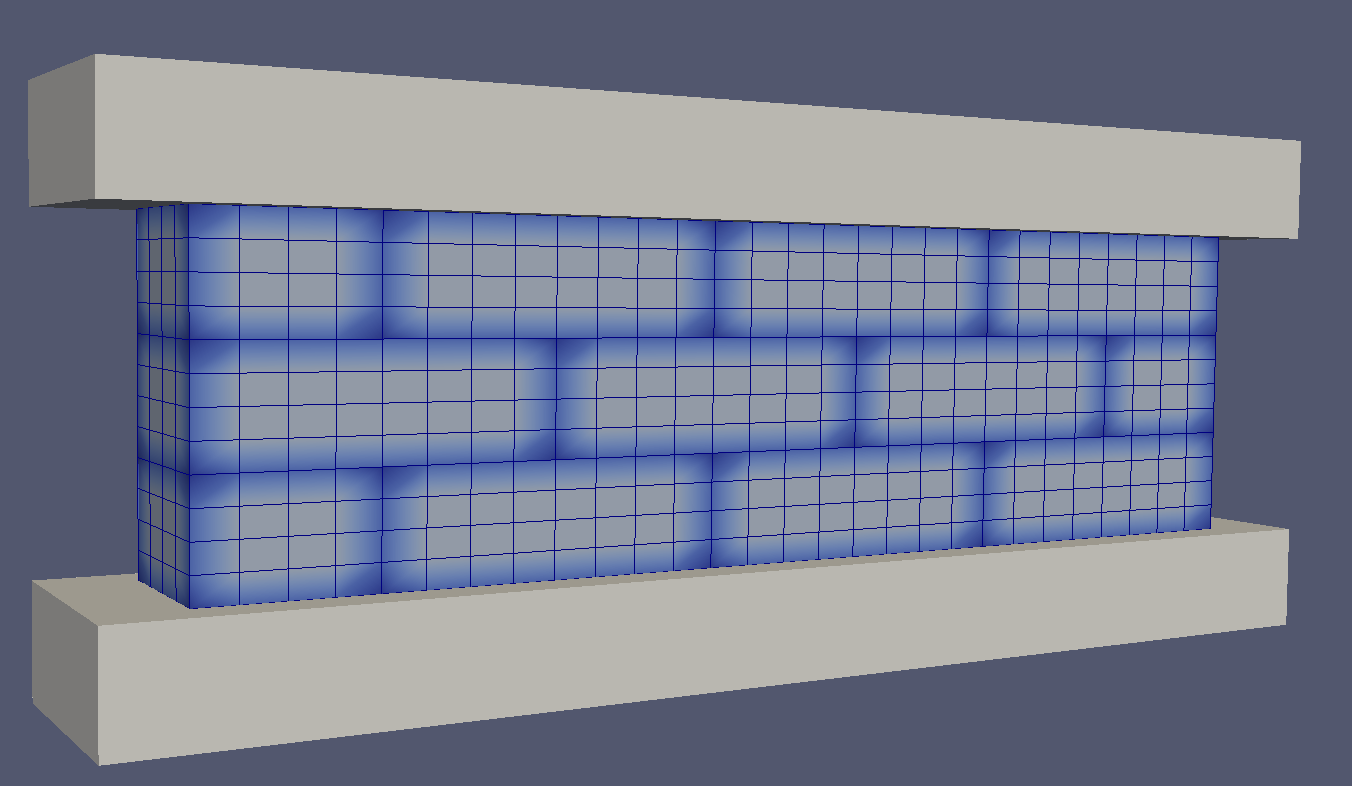
\includegraphics[height=0.5\textheight]{../figure/LowWall_FEM.png}
  \caption{A low wall meshes with H8}
  \label{fig:LowWall_FEM}
\end{figure}
\vspace{-0.5cm}
\begin{itemize}
\item H8 FE with Linear elastic behavior :
  $\rho= \num{2000}\si{\kilogram\per\cubic\metre},
  E=\num{2.2e+9}\si{\pascal} ,\nu = 0.2$
\item $\mu= 0.83 $ between block and $\mu =0.53$ between blocks and supports
\item Vertical compression force : $30000 \si{\newton}$ horizontal shear velocity $\num{1e-3}\si{\meter\per\second}$.
\item Sampling of $50$ problems collected in the FCLib with graded difficulty 
\end{itemize}
\end{frame}



\begin{frame}
  \frametitle{Results}
  \begin{figure}[htbp]
    \begin{center}
  \centering 
  \subfloat[Accuracy $\epsilon = 10^{-2}$]{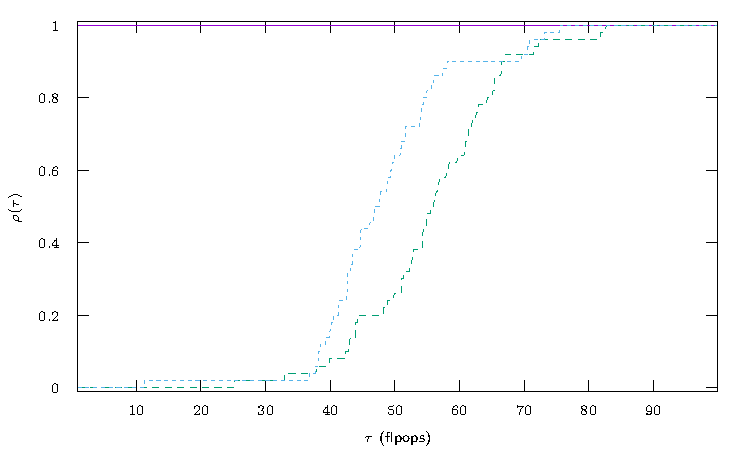
\includegraphics[width=0.55\textwidth]{../figure/LowWall_FEM.1e-2.with_guess/simple/profile-LMGC_LowWall_FEM.pdf}\label{fig:LowWall_FEM.1e-2.simple}}
   \subfloat[Accuracy $\epsilon = 10^{-3}$]{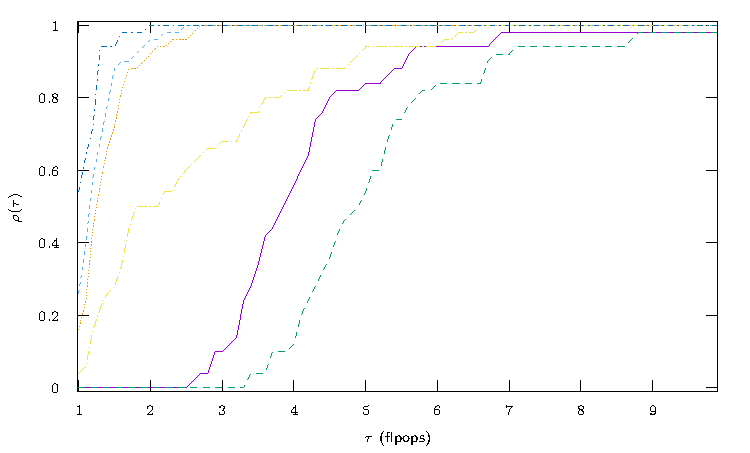
\includegraphics[width=0.55\textwidth]{../figure/LowWall_FEM.1e-3.with_guess/simple/profile-LMGC_LowWall_FEM.pdf}\label{fig:LowWall_FEM.1e-3.simple}}\\
   %\subfloat[Accuracy $\epsilon =  10^{-4}$]{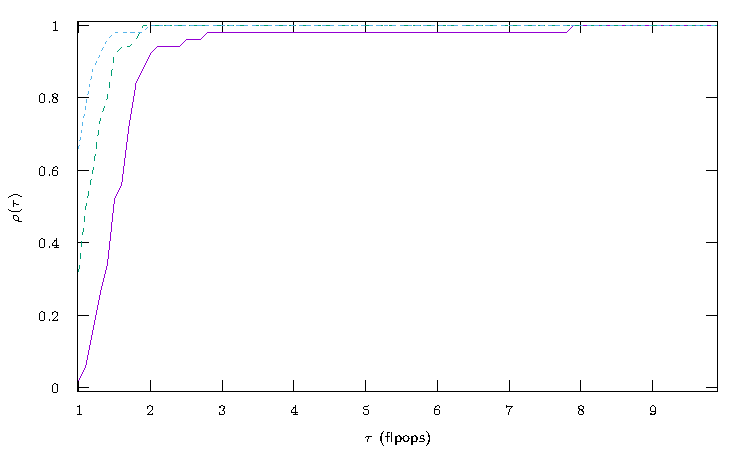
\includegraphics[width=0.49\textwidth]{../figure/LowWall_FEM.1e-4.with_guess/simple/profile-LMGC_LowWall_FEM.pdf}\label{fig:LowWall_FEM.1e-4.simple}}
   %\subfloat[Accuracy $\epsilon = 10^{-6}$]{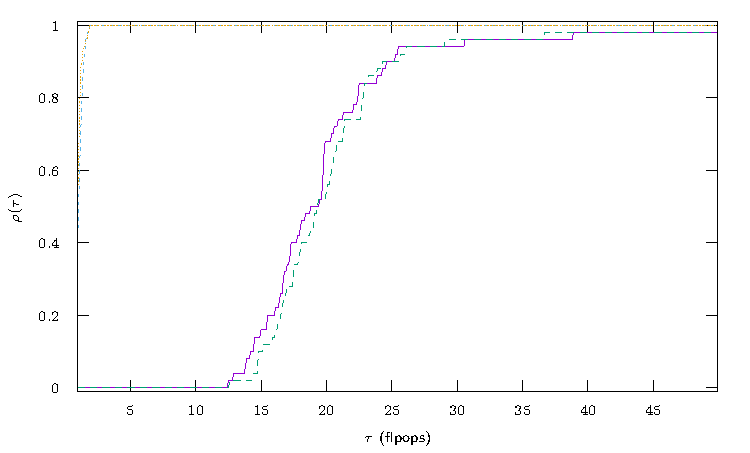
\includegraphics[width=0.49\textwidth]{../figure/LowWall_FEM.1e-6.with_guess/simple/profile-LMGC_LowWall_FEM.pdf}\label{fig:LowWall_FEM.1e-6.simple}}\\
   % \subfloat[précision $\epsilon = 10^{-8}$]{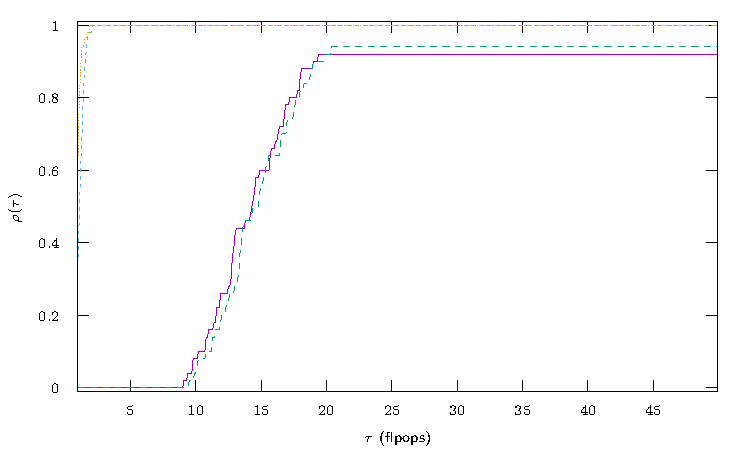
\includegraphics[width=0.49\textwidth]{figure/LowWall_FEM.1e-8.with_guess/simple/profile-LMGC_LowWall_FEM.pdf}\label{fig:LowWall_FEM.1e-8.simple}}\\
   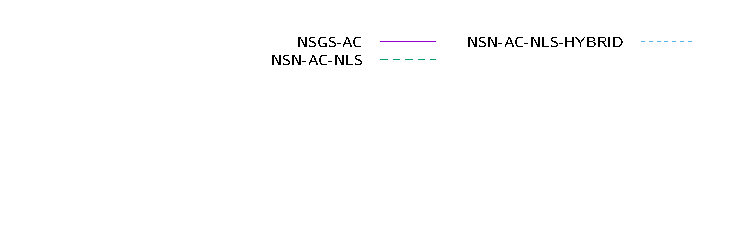
\includegraphics{../figure/LowWall_FEM.1e-2.with_guess/simple/profile-LMGC_LowWall_FEM_legend.pdf}
 \end{center}
  \caption{Comparison for two different required accuracies}
  \label{fig:LowWall_FEM.simple}
\end{figure}
\end{frame}

\begin{frame}
  \frametitle{Results}
  \begin{figure}[htbp]
  \centering 
  %\subfloat[Accuracy $\epsilon = 10^{-2}$]{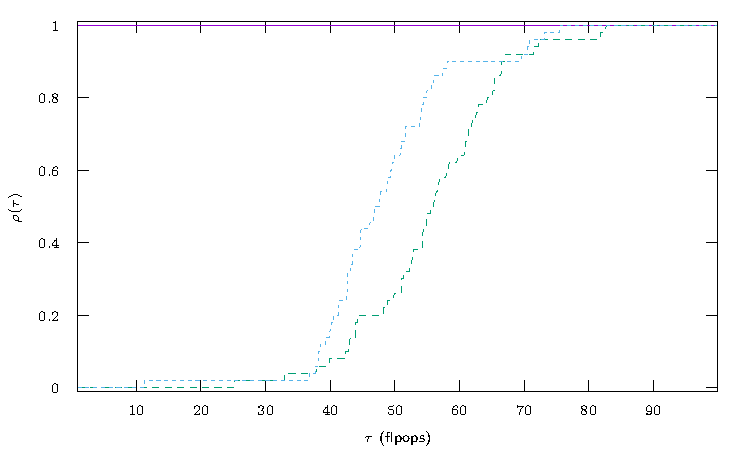
\includegraphics[width=0.49\textwidth]{../figure/LowWall_FEM.1e-2.with_guess/simple/profile-LMGC_LowWall_FEM.pdf}\label{fig:LowWall_FEM.1e-2.simple}}
  % \subfloat[Accuracy $\epsilon = 10^{-3}$]{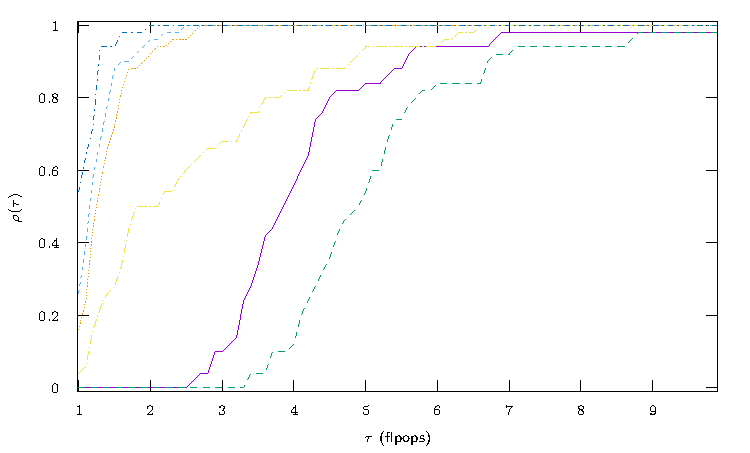
\includegraphics[width=0.49\textwidth]{../figure/LowWall_FEM.1e-3.with_guess/simple/profile-LMGC_LowWall_FEM.pdf}\label{fig:LowWall_FEM.1e-3.simple}}\\
   \subfloat[Accuracy $\epsilon =  10^{-4}$]{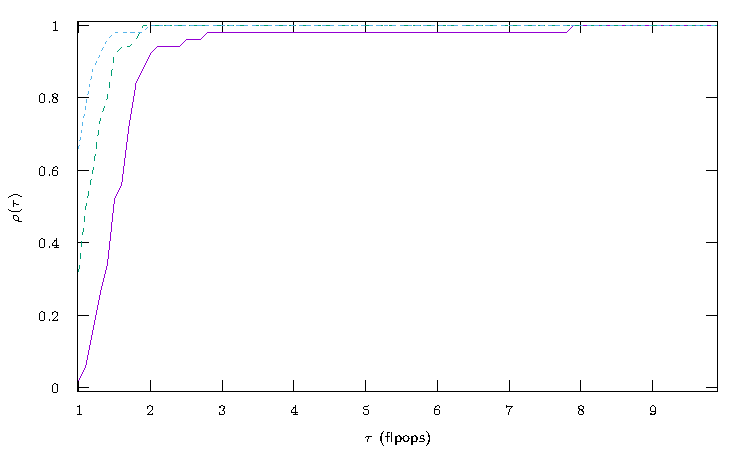
\includegraphics[width=0.55\textwidth]{../figure/LowWall_FEM.1e-4.with_guess/simple/profile-LMGC_LowWall_FEM.pdf}\label{fig:LowWall_FEM.1e-4.simple}}
   \subfloat[Accuracy $\epsilon = 10^{-6}$]{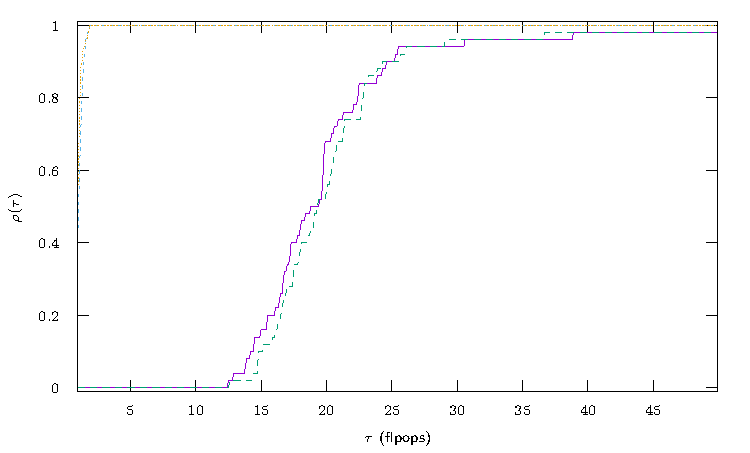
\includegraphics[width=0.55\textwidth]{../figure/LowWall_FEM.1e-6.with_guess/simple/profile-LMGC_LowWall_FEM.pdf}\label{fig:LowWall_FEM.1e-6.simple}}\\
   % \subfloat[précision $\epsilon = 10^{-8}$]{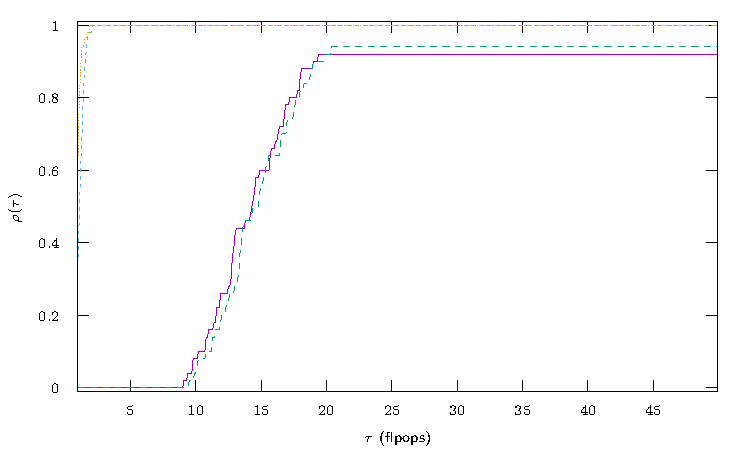
\includegraphics[width=0.49\textwidth]{figure/LowWall_FEM.1e-8.with_guess/simple/profile-LMGC_LowWall_FEM.pdf}\label{fig:LowWall_FEM.1e-8.simple}}\\
   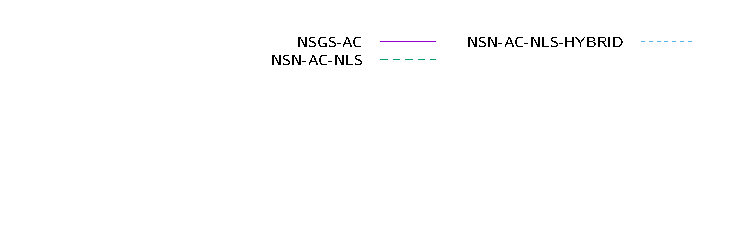
\includegraphics{../figure/LowWall_FEM.1e-2.with_guess/simple/profile-LMGC_LowWall_FEM_legend.pdf}
  \caption{Comparison for two different required accuracies}
  \label{fig:LowWall_FEM.simple}
\end{figure}
\end{frame}
%%% Local Variables:
%%% mode: latex
%%% TeX-master: "s"
%%% End:










\section{Conclusions \& Perspectives}
\frame{
\frametitle{Conclusions \& Perspectives}
\begin{block}{Conclusions}
  \begin{enumerate}
  \item For relatively tight accuracy, nonsmooth Newton methods outperform first order iterative methods.
  \item  {\sf\small NSN-AC-NLS-HYBRID} is the most efficient method
  \item First order iterative methods are interesting for low accuracy, but are not able to reach tight accuracy,
  \end{enumerate}
\end{block}
\vskip-3mm
\begin{block}{Perspectives}
  \begin{enumerate}
  \item Evaluate the interest to transform rigid model into flexible ones.
  \item Study the possibility to take into account the possible nonlinear bulk behavior in the Newton loop
  \item HPC and scalability  of nonsmooth Newton techniques using MUMPS 
  \item Continue to set up a collection of benchmarks  \ding{220} FCLIB
  \end{enumerate}
\end{block}

}

\subsection{FCLIB : a collection of discrete 3D Frictional Contact (FC) problems}

\frame{
  \frametitle{FCLIB : a collection of discrete 3D Frictional Contact (FC) problems}
  Our inspiration: MCPLIB or CUTEst
  \begin{block}
    {What is FCLIB ?}
    \begin{itemize}
    \item A open source collection of Frictional Contact (FC) problems
      stored in a specific HDF5 format 
    \item A open source light implementation of Input/Output functions
      in C Language to read and write problems (Python and Matlab coming soon)
    \end{itemize}
  \end{block}


  \begin{block}
    {Goals of the project}
    Provide a standard framework for testing available and new algorithms for solving discrete frictional contact problems share common formulations of problems in order to exchange data
\end{block}
\begin{block}
    {Call for contribution}
    \alert{\url{http://fclib.gforge.inria.fr}}
  \end{block}
}

\frame
{
\centerline{\textcolor{red}{ Thank you for your attention.}}
}

\def\newblock{}
{\scriptsize
\bibliographystyle{plain}
\bibliography{biblio}
}

%\include{PWL}


\end{document}

%%% Local Variables: 
%%% mode: latex
%%% TeX-master: t
%%% End: 
